	\chapter{Optimizing Application Performance through Autoscaling Policies}  
  \label{ch:optimization-virtualized} 
  In chapter \ref{ch:optimization}  we analyzed the end-to-end  Management of service center, where number of service replicas and placement of these replicas was obtained by solving a single optimization problem.  
 Using virtualization, it is possible to offer infrastructure in terms of small chunks, namely virtual machines. As a IaaS user, we use the virtual machines as unit's of hardware with isolated and consistent performance attributes. The infrastructure as a service (IaaS) layer   solves the placement problem for virtual machines on available hosts in a way that it satisfies hardware layer goals regarding consolidation or homogeneous utilization. Thus, one can use IaaS and focus on provisioning of services using virtual machines.  

 \section{The Formulation}
Lets assume virtual machines are grouped into a set of $Cl$ clusters based on services they host. Each cluster is homogeneous; % in the sense that every virtual machine within a cluster meaning that it hosts the same set of services that has the same virtual machine specification. Each service can span multiple clusters. Let us assume  $m_{cl}$ represents the number of machines in cluster $cl$.  
   Recalling from chapter \ref{ch:optimization}, the physical workload imposed on resource $k'$ of host $h$ from customers of class $c$ accessing service $s$ is calculated by the expression: $X_c (V_{c,s} \theta_{s,h}) D_{s,k'}$.   Further, let's assume within each cluster $cl$ the resource usages are distributed equally between all the hosts  ($\theta_{s,h}$ are equal  for each cluster). With these assumptions, each cluster can be modeled as a shared queue multi-server, which can be approximated, by a queuing centre and a delay centre. The new service demands of the cluster are then derived as $d_{c,s}\theta_{s,cl}= V_{c,s} D_s \theta_{s,cl}$. 
   
   To further simplify the problem, let us assume all the classes in the system are aggregated into one class. Then the high level objectives can be described in terms of aggregated throughput $X$ and response time $R$.   % As a result demand of each service on that type of virtual machine is only indexed by the service, $D_s$.  In addition, in this case, on each virtual machine a single replica of a service is deployed. 
  Then targeting only cluster $cl$, demand of each cluster can be derived as sum of the demands of services deployed on the cluster considering the the multi-cluster services 
  $d_{cl}=\sum_s d_{c,s}\theta_{s,cl}$.    % $d_{cl}=\sum_s d_{s,cl}$. 

%  instead of  service demands in terms of class–service–resource type
%   in this chapter we index demand in terms of class–cluster–resource type. 
% 
%  instead of $D_s$ which includes $d_{c,s}=V_{c,s} D_s$  and gets  distributed  
%  between hosts as $d_{c,s,h,k'}=X_c (V_{c,s} \theta_{s,h}) D_{s,k'}$, 
%  
%   where cl is considered a multi-server shared queue resource. 
  

  \section{Sub-Optimal Autoscaling through Utilization Control}   % Stationary Policy  
 %  \subsection{suboptimal solution  heuristic PID utilization control}  
  \label{sec:non-optimal-autoscaling}   
 
   Utilization control as a way to regulate high-level performance metrics such as throughput has been investigated in different contexts than service centre autoscaling \cite{kalyvianaki_self-adaptive_2009}.  In this subsection, we propose solving the autoscaling problem in service centre using the simplistic utilization control.
    The intuition behind this approach is that if increasing multiplicity of a cluster improves the overall throughput, then the utilization experienced by every server in the cluster after autoscaling will not drop as much. This is because increase in the multiplicity is compensated with the extra throughput to be handled. If the autoscaling action has no effect on throughput, the load each individual server in the cluster experiences after scale-up is going to decrease proportional to the increase in the number of added resources. 
       
%   note that the relationship between the utilization and the multiplicity of a resource described as follows:  
%       (i) When a resource is a bottleneck, adding to its multiplicity will result in improving the overall throughput, but utilization of the resource will not drop  while it is the bottleneck. 
%      (ii)  when a resource just exists the bottleneck status, its utilization will drop with addition of its multiplicity. This behaviour follows the formula $U=XD_{\text{queuing}}+XD_{\text{delay}}$. increasing the multiplicity of this resource  does not increase system throughput but lowers the demand   of the  approximated queuing centre and thus utilization of multi-server.     
%      (iii)   After the queue length on the approximated queuing centre goes towards 0, 
%      the utilization of the multi-server goes towards the delay centre's utilization, 
%      $U=XD_{\text{queuing}}+XD_{\text{delay}}$.  
  
  % if a service is a bottleneck then its service rate is low but utilization is low means its a  software bottleneck.
 

%\section{Non-Optimal  Autoscaling of Aggregated Class Workloads}   % Stationary Policy  
%\label{sec:non-optimal-autoscaling}
%
% \textbf{The objectives} of the  lower control  layer are as follows: 
% 
% (1)  \textbf{regulating the  average utilization of  resources} around certain value such as 60\%.  
%   Regulating a  utilization of  a single resource around such value guarantees that the resource is not a bottleneck 
%    for services deployed  on it. In this case the objective function will contain a term denoting a norm of deviation from the target  utilization for  hardware resources  of each host: $\text{minimize} \sum_{t'=1}^{T'} \sum_h (U_{h,t} - 0.6 \capp_h)$). The other way to model the objective is to aggregate utilization of all the hosts into a single distribution and encode the objective in terms of mean and variance of this distribution  (i.e. the distribution of the probability of the machine having certain resource utilization (i.e. $P(\frac{U_h}{\Omega}=U_0)$) obtained from  the current  utilization  level  of hosts (i.e. $\frac{N(\frac{U_h}{\Omega}=U_0)}{H}$ ).  The variance of this distribution   represents the homogeneity of the infrastructure utilization.  Since a target is having a homogeneous cluster or cloud in terms of resources utilization, the target should be minimizing this variance.  Note that there is a trade-off between minimizing the variance of the resource utilizations and the amount of trashing done through change of service books. Also, note that the variance in black box case depends on the performance of the placement algorithm.
   
%  (2) Range Regulation: The controller can also try to regulate the resource utilizations in the range of values rather than around a single point target  (for example between 50\% and 70\%).  In this case the objective function will contain a term that penalizes the excess of the utilization over the upper bound and its shortage below the lower bound: $  \text{minimize} \sum_h \mathtt{pos}(U_h-0.7) + \mathtt{pos}(0.5-U_h) $. In case of the distribution, this objective is the present by putting certain percentile (such as 51\%) of the distribution into the interval 
%  The dynamics of and system and out the autoscaling part are as follows. 

 % one of the current techniques used in industry to manage overall performance  of applications is autoscaling single services based on  some stationary policy.  Although widely used, formalization of this type of policy and its effect on the system performance is not investigated thoroughly. 
 
 % In this subsection to provide the formalization of this type of policy, which can be used as a baseline to be compared to other suggested approaches.
  
    In such system, the end-to-end throughput goal is satisfied if no service is a bottleneck.  Assuming that the multiplicity of software services are high enough not to cause a software bottleneck, the necessary and sufficient condition to satisfy end-to-end throughput goals is that the underlying hardware resources supporting the service are not saturated. By lowering the utilization enough (i.e. 60\%) it is guaranteed that hardware throughput at least equal to the SLA throughput.   
    
    Note that for each service a different type of resource might be the bottleneck for example for database service usually the memory or disk, for a load balancer service the network, and for the application logic services the CPU is a bottleneck. 
     For the cluster that hosts multiple services, finding the bottleneck resource before the deployment is not feasible. Thus at runtime, one has to set the controller targets around the bottleneck resource. In case of multiple bottleneck resources controller should maintain multiple targets (we do not cover this case here.).  
   
         We propose a simple way for controlling the utilization of the cluster using a PID like controller system. Dynamics of such controller system are as follows: 
         \begin{align} 
              x=f(x,\Delta U) \\ 
              y=g(x)
           \end{align}    
  here deviation of system outputs (resource utilizations)  from desired outputs $\Delta U=U^{\text{target}}-U$  is the input to the controller system, and $x$ is the state of the controller.  Note that the output of the controller in each time step depends on past outputs of the system as well as the current one.  
  
   Let's assume $U_{cl,h,k',t}$  represents the utilization of resource type $k$ of host $h$  of cluster $cl$ at time $t$. Then the extent to which a utilization has been breaching a specified threshold is denoted by
    \begin{align}  
      \Delta U_{cl,h,k',t}=U^\text{target}_{cl,k'}-U_{cl,h,k',t}
    \end{align} 
  Lets assume we define a smoothing state 
  \begin{align}  
   \Delta U^\text{smoothing}_{cl,h,k',t} = \alpha_{cl,k'} \Delta U^\text{smoothing}_{cl,h,k',t}+(1-\alpha_{cl,k'})\Delta U_{cl,h,k',t}   
   \end{align} 

   were $\alpha\in[0,1]$  that accumulates the history of utilization breachings of the past.
 The idea is that the autoscaling action for cluster $cl$ at time $t$ is derived by aggregating the tensor $\Delta U^\text{smoothing}_{cl,h,k',t}$ over resource types $k'$  and hosts $h$. Here we aggregate over the resource types of each host by summing the smoothing state:   
\[
\xi_{cl,h,t}=\sum_{k'} \Delta U^\text{smoothing}_{cl,h,k',t} 
\]   
 and aggregate over the hosts  by taking  majority vote: %50 percentile
\[
  \kappa_{cl,t} = \left\{    
  \begin{array}{l l}
    \text{acquire} & \quad \text{if $\left(\sum_{j=1..N} \xi_{cl,h,t}\right)/N > \mathtt{d}$}\\
    \text{release} & \quad \text{if $\left(\sum_{j=1..N} \xi_{cl,h,t}\right)/N < \mathtt{d}$}\\
    \text{none} & \quad \text{otherwise} 
  \end{array} \right. 
\]

%Although this controller can be used to constrain the utilization the cluster in an operating region, it has two problems:  
 %(i) Controller does not take into account the cost of resources. The resource cost is an implicit side effect of the configuration of the controller. Section ... introduces our new approach to autoscaling that considers the cost.  
 %
  %(ii) There is no automatic way to find the proper number of alerts, and the associated values for \texttt{a},\texttt{e},\texttt{d} based on the properties of the controller.  However informally we can summarize the effect of these parameters. 
    %
=============
\subsection{implementation through rule-based systems}
one way to specify the above controller is through rule-based systems.
As far as we are aware, the only publicly available rule-based provisioning solution implemented for the cloud is RightScale platform \cite{rightscale_autoscaling}).
Rules are specified as follows:  'if \textit{condition} then \textit{action}' where the \textit{condition} represents a term defined recursively based on the value(s) of monitored metric(s)\footnote{A condition can be a conjunction or disjunction of other conditions}.   
An \textit{action} might involve the realization of a global management decision (e.g. adding or removing servers), a local management decision  (e.g. increasing a process's memory), or emitting an event (e.g.,  an {\it alert}). 
Further, an implicit target exists for the types of  management rules.  For example, in a transactional application the target might be an individual server. % Monitored metrics might also vary based on the alert target. 

\begin{figure}[b]
	\centering
	\includegraphics[width=0.45\textwidth]{image/loop/controller-rule-based.eps} 	
	\caption{Architecture of a rule-based autoscaler.}
	\label{fig:rule-based-resource-provisioner}
\end{figure}

In a rule-based autoscaler the process of deriving global provisioning decisions using the locally fired rules of individual servers is as follows:
if a rule specification's \textit{condition} holds for longer than the defined \textit{decision\_duration} in the rule's target, an alert is triggered from that target. 
If the associated target is eligible, it will then vote for performing the specified action. 
Once the number of targets voting to grow exceeds a specified \textit{decision threshold} (e.g. 51\%) a scaling action will be performed. 
If, after resizing, the number of instances falls within the interval defined between \textit{min\_instances} and \textit{max\_instances} a scaling action will launch/terminate a number of instances configured by a \textit{resize number}. Once a scaling action occurs, the system is not allowed to perform another scaling action until a \textit{refractory period} has passed. This is because, it takes some time to launch a new server (i.e. copying the server image to a physical host and booting a VM from it) 
before it becomes operational and starts offloading some of the work from the overworked instances. 
If these additional servers make enough impact, the triggered alerts in some targets disappear, the number of votes decreases below the decision threshold and autoscaling will be stopped. Otherwise, after the refractory period, a new autoscaling action will be triggered again. 

The conditions which result in an alert being issued are defined based on various metrics. 
In a typical transactional system one can use hardware level metrics of each host, process level metrics of each operating system process, 
and service specific metrics for different types of servers (e.g. load balancer, web server, application server, and database server). 

A template of an alert specification for a transactional system is presented in Table \ref{tab:alerts-spec-example}. 
Using the alerts of Table \ref{tab:alerts-spec-example}, one can configure an autoscaler to launch an additional instance when a majority of the servers are being overworked and then to remove an instance when servers are underutilized due to a decline in traffic.  
In this example, adding multiple alerts defined based on multiple metrics is also possible . For example, for an application which is both memory and CPU intensive at times, one can set up alert specifications based on both CPU utilization and available memory. 

   %\texttt{quorum}         & 51\% & 51\% & 51\% \\
   %\texttt{refractory\_period} & 8 min & 8 min & 6 min \\
	
\begin{scriptsize}
\begin{table}[b]
\center
\begin{tabular}{ |l|l|l| }
\hline 
Condition & Duration & Action \\
\hline \hline 
If \texttt{cpu-idle} $<$ \texttt{cpu\_idle\_gt} &  \texttt{grow\_duration}  & vote to \texttt{grow} by \texttt{incr\_val}  \\
If \texttt{cpu-idle} $>$ \texttt{cpu\_idle\_st} &  \texttt{shrink\_duration}  & vote to \texttt{shrink} by \texttt{decr\_val} \\
\hline 
\end{tabular}
	\caption{Template of alert specifications.}
	\label{tab:alerts-spec-example}
\end{table}
\end{scriptsize}

There are various ways that one can configure an autoscaler. 
For example, for a transactional application deployment with $l$ hosts, $m$ available metrics, and $n$ predicates for defining conditions,
 each host might choose a subset of $[\text{predicates} \times \text{metrics}]$ (i.e. $2^{n*m}$ choices) to define its alerts.
These alternatives, together with global configuration parameters \textit{decision threshold}, \textit{resize number}, \textit{min\_instances}, and \textit{max\_instances} form a huge configuration space and this makes it hard to investigate each configuration parameter's impact on the behavior of the autoscaler.    

%One way of characterizing an autoscaler's behavior is to show how it reacts to the perturbations in the environment (i.e., disturbance input to the system). 
%Rather than accessing the effectiveness of an autoscaler in achieving objectives defined on system output(s) this characterization helps in comprehending autoscaler behavior in general. 
%One can aim at building mathematical model for behavior of the autoscaler.
%For example by considering autoscaler decision (i.e. here number of instances) over time as a transfer function $F(z)$ over configuration parameters (i.e. subset of predicates applicable to system outputs) and system output (e.g. average server utilization): 
%\[\text{servers}(z) = F_\text{configuration}(z) \text{sys-out-metric}(z)\] 
%servers = f(configuration,utilization)
% knowing that autoscaler decision together with workload component make inputs of the system $G(z)$: 
%\[\text{sys-out-metric}(z) = G(z)[\text{servers}(z)+\text{workload}(z)]\] 
%utilization = g(servers,workload)
%one might be able to construct a transfer function $H(z)$ from workload component to the autoscaler decision (for a specific system)
%\[\text{servers}(z)=H_\text{configuration}(z)\text{workload}(z)\]
%servers=f(configuration,g(servers,workload))
%The approach we took in this work was to roughly characterize autoscaler based on its decisions (over configuration space) rather than modeling it formally. 
% roughly derive properties of
% We considered autoscaler as a transfer function which takes the workload function and maps it to a function representing number of active instances over time (lets call it \textit{node curve}). 
% We consider the autoscaler as a transfer function which takes the workload and maps it to a function representing the number of active instances over time (i.e., a {\it node curve}).   
%Next, we qualitatively categorized the effect of each configuration parameter on this transfer function.
%To further simplify it, we assumed there is only one subsystem under autoscaling (e.g. application server tier) with homogeneous instance types and CPU utilization is the only metric used in defining alert types.

In our experiments all the alerts in all targets were identical and based on the template introduced in Table \ref{tab:alerts-spec-example} (e.g., two alerts where defined, one for scale-up action is case of over-utilization and one for scale-down in case of under-utilization).
Over-utilization is considered when CPU idle time is less than the lower bound \textit{cpu-idle-lb} and underutilization is defined as when CPU idle time is more than the upper bound \textit{cpu-idle-ub}.
The interval $[\text{\textit{cpu-idle-lb}},\text{\textit{cpu-idle-ub}}]$ formed by these two bounds, together with {\it decision threshold}, {\it refractory period}, {\it decision durations}, {\it resize numbers}, and $[\text{{\it min\_instances}},\text{{\it max\_instances}}]$ interval form a simpler configuration space that we investigate in this work. 
We summarize the effect of different autoscaler configurations on the scaling behavior in the next subsection.

   \subsection{Informal Description of Controller Configuration Effects}
We consider the autoscaler described earlier as a transfer function, which takes the output of a service cluster and maps it to actions governing size of the cluster over time.    
Next, we qualitatively categorized the effect of each configuration parameter on this transfer function.

In our experiments all the alerts in all targets were identical and based on the template introduced in Table \ref{tab:alerts-spec-example} (e.g., two alerts where defined, one for scale-up action is case of over-utilization and one for scale-down in case of under-utilization).
Over-utilization is considered when CPU idle time is less than the lower bound \textit{cpu-idle-lb} and underutilization is defined as when CPU idle time is more than the upper bound \textit{cpu-idle-ub}.
The interval $[\text{\textit{cpu-idle-lb}},\text{\textit{cpu-idle-ub}}]$ formed by these two bounds, together with {\it decision threshold}, {\it refractory period}, {\it decision durations}, {\it resize numbers}, and $[\text{{\it min\_instances}},\text{{\it max\_instances}}]$ interval form a simpler configuration space that we investigate in this work. 
We summarize the effect of different autoscaler configurations on the scaling behaviour as follows:

%\begin{description}
\textbf{Operating interval} formed by $[\text{\textit{cpu-idle-ub}},\text{\textit{cpu-idle-ub}}]$ is the main tool in configuring the long term size of the cluster. 
It basically forces the autoscaler to act until the cluster reaches the desired average operating interval (here in terms of CPU idle time, e.g. $[20\%,30\%]$ idle).

If the desired operating interval is located at high CPU idle values (e.g. $[40\%,50\%]$), there will be a lot of instances launched.
Autoscaling will eventually stop due to the increase in the number of idle instances, resulting in less alerts being signaled (as the triggering threshold is no longer reached). 
Notice that the autoscaling action is only performed if the intensity of the workload can get cluster nodes to the desired operating point. Thus, if 
the operating point is configured when nodes are fully utilized (e.g. $[0\%,10\%]$ CPU idle time), the cluster might become unresponsive for low intensity workloads.

If this interval is configured to be narrow and it is placed in an operating area reachable by the workload, it will make the autoscaler sensitive to changes. Such an autoscaler would do some thrashing just to keep the operating point at this narrow interval. If the interval is wide, the cluster will be less responsive, and the cluster utilization will have more space for variations. 

\textbf{Decision duration} contributes to the responsiveness of the cluster. A shorter decision duration for each node results in a quicker response and, thus, it is better at detecting highly variable workloads (e.g. a workload that changes direction every 15 minutes). 
 In case of steady or monotonically increasing/decreasing workloads, the cluster is going to stabilize on a specific size no matter what decision duration is. 

\textbf{Resize numbers} represents the amount of servers to add or remove should a decision threshold (i.e., quorum) be reached  (e.g., 51\%). 
This has a short-term effect on the size of the cluster by making it grow or shrink faster. This might be useful for heavily increasing or decreasing workloads. However, in a long run for a lightly changing workload this might only have effect on smoothness of cluster size over time. 

\textbf{Decision threshold} is global parameter closely related to decision duration, which can affect the responsiveness of the cluster specially in a heterogeneous clusters.
In a heterogeneous cluster, nodes with less processing power might reach the saturation level faster. In this case, a lower decision threshold might result in a better autoscaling decision. The same applied to cluster composed of two different types of nodes (e.g. front-end and application server) where the load on one type of node is higher than the other (e.g. a web application with lots of demand on static resources would result into more utilization at the front-end). 

\textbf{Instance bounds} formed by $[\text{{\it min\_instances}},\text{{\it max\_instances}}]$ acts as constraint on the size of the cluster. 

\textbf{Refractory period} is the interval of time which follows an autoscaling action during which no autoscaling actions may occur.  
% can determine how well the cluster can resize for a changing workload. 
With small refractory periods, the cluster makes resizing decisions more frequently resulting in behavior that is more responsive. 
% \end{description}
%
%\begin{figure}[htb]
	%\centering
	%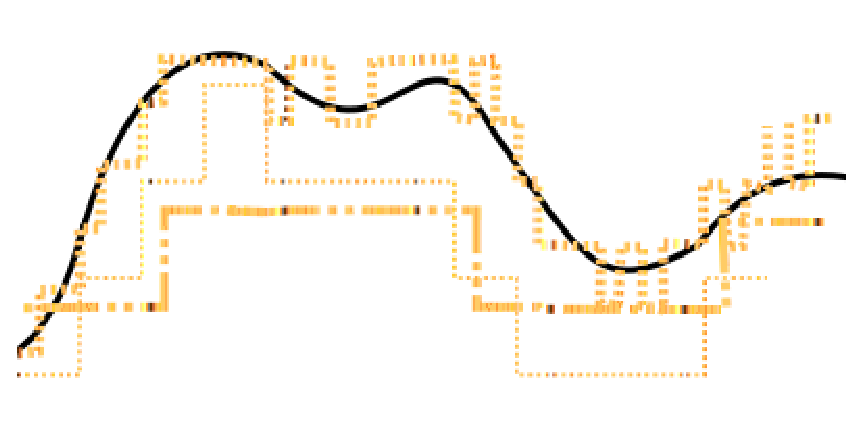
\includegraphics[width=0.45\textwidth]{./image/pre/workload6.eps}
	%% workload6.eps: 0x0 pixel, 300dpi, 0.00x0.00 cm, bb=14 14 413 207
	%\caption{Effect of different autoscaler configurations on the scaling behavior.}  
	%\label{fig:different-autoscaler-configuration}
%\end{figure}
%
%Figure~\ref{fig:different-autoscaler-configuration} schematically represents the behavior of three different autoscaler configurations on the scaling behavior. The workload is represented by a solid line, while the number of instances (an a representative of autoscaler behavior) in three different configurations is represented by step-like functions. 


\subsection{An Example} 
Here we show the results of applying different elasticity policies on the same workload an application. the architecture for the application will be discussed in detail in section ... only note that  auto-scaling actions are applied to the application server tier.

The workload used (see figure \ref{fig:scenario_workload}) is FIFA '98, Day 41, partial excerpt.  
 \begin{figure}
   \centering
    \label{fig:workload41partial}\includegraphics[height=2.1in,width=3.2in]{himgs/fig3/img1}
    \caption{FIFA '98, Day 41, partial excerpt.}
		\label{fig:scenario_workload}
 \end{figure} 
	
 Three different elasticity policies were designed to drive the auto-scaling actions of the application server tier under different circumstances. These policy sets utilized different settings of some of the configurable parameters mentioned above and are presented in Table~\ref{tab:ps}.   %They were designed through trial and error.  
 
  The first elasticity policy, $P_\text{Sensitive}$, was designed to be gentle in how it grew/shrunk the tier (i.e., adding/removing only one platform instance at a time).  % $S_0$
Similarly, the second elasticity policy, $P_\text{tolerant}$, increased and decreased the topology in a gentle fashion as well; however, the range separating its two thresholds (upper and lower) was three times as large as for $P_\text{Sensitive}$ making it much less likely to be triggered as often (assuming violations occur inside the defined range). 
%  $S_1$ 
The third elasticity policy, $P_\text{Aggressive}$, was designed to be much more aggressive in how it grew/shrunk the tier as evidenced by both a small range between its upper and lower thresholds and an increment value (up and down) of two.  % $S_2$
 
\begin{table}[h]
\caption{Parameter settings defining the three elasticity
policies. The values for $\texttt{grow\_duration}$, $\texttt{shrink\_duration}$ and $\texttt{refractory\_period}$ are the actual values used in the experiment (i.e., scaled by one quarter).}\label{tab:ps}
\center
\begin{tabular}{ ||c || c | c | c| }
  \hline
   Parameter & $P_\text{Sensitive}$ & $P_\text{Tolerant}$ & $P_\text{Aggressive}$ \\
   \hline \hline                       
   \texttt{incr\_val}      & 1 & 1 & 2  \\
   \texttt{decr\_val}      & 1 & 1 & 2  \\
   \texttt{quorum}         & 51\% & 51\% & 51\% \\
   \texttt{cpu\_idle\_gt}  & 45   & 40   & 50   \\
   \texttt{grow\_duration} & 7 min & 7 min & 8 min \\ 	
   \texttt{cpu\_idle\_st}  & 50 & 55 & 55 \\
   \texttt{shrink\_duration} & 7 min & 7 min & 8 min \\
   \texttt{refractory\_period} & 8 min & 8 min & 6 min \\
  \hline  \hline
\end{tabular}
\end{table}

From figures \ref{fig:scenario_number_of_sessions} and \ref{fig:scenario_additional_platform_instances}, notice that the differences in both total sessions and additional platform instances utilized over time varies substantially among the three approaches.   
   

	\begin{figure}
   \centering	
    \label{fig:csps123}\includegraphics[height=2.1in,width=3.2in]{himgs/fig3/img2fill}
  \caption{ Number of sessions processed by the application in response to the workload using
 three alternative elasticity policies (EP)s.  }
\label{fig:scenario_number_of_sessions}
 \end{figure} 

	\begin{figure}
   \centering
    \label{fig:ipps123}\includegraphics[height=2.1in,width=3.2in]{himgs/fig3/img3}
 \caption{ Additional platform instances being added and released in response to the workload under the three alternative EPs.}
\label{fig:scenario_additional_platform_instances}
 \end{figure} 
  
 %{imgsCNSM2011/day41-rp}
    %\\
 %{imgsCNSM2011/cs_p123}}
    %\\
    %\hspace{0.5in}  
 %{imgsCNSM2011/pi_p123}}



\section{Switching Policies}
\label{s:switching-policies}
In order to achieve better results  in a long run, one can heuristically switch between different short-term policies 
by repeatedly evaluating the high-level objectives. 
For example, in our case, although the autoscaler is only capable of regulating the cluster utilization, we can still assess the policies for high-level objectives such as:
 (i) maximizing the number of clients serviced. 
 (ii) keeping the mean response time at or below some threshold.  
(iii) limiting the number of additional platform instances purchased.
	
	Let us assume that the three policies introduced earlier are the only possible set of choices. 
	$P_\text{Aggressive}$ over-provisions aggressively at all times. Applying this policy makes sense if a flood of clients is detected. $P_\text{Sensitive}$ involves careful and slow provisioning which is beneficial in periods of sporadic and/or limited usage. $P_\text{Tolerant}$ attempts to under-provision by some percentage. 
	
	The management unit would monitor  and store high level metrics such as number of sessions, response time, and number of instances purchased over time. At certain intervals (which we call epoch) the management would choose which policy should be employed as the active one. we chose one hour an epochs. Since The monitoring framework lets us measure things as frequently as every four minutes, there will be 60 samples (4* 15) available per epoch (for each of the metrics including number of sessions and number of purchase instances). 
This data in combination with the current active policy denotes the {\it state}. 

	The decision on the next policy will essentially depend on this state. 
	This decision would be based first upon the detection (or lack of detection) of a trend in the number of current sessions observed over the previous epoch. Two trends were identified as being of interest:  steeply increasing (SI) and steeply decreasing (SD). Should no strong trend be detected, data about the additional purchased platform instances for the previous four hour epoch would then be utilized.
	
  %Current == S_0
  If the current active  policy is $P_\text{Sensitive}$ the following reasoning is used.
  If steep increase or decrease in the number of sessions is observed then the next policy is set to $P_\text{Aggressive}$ in order to ensure that available resources are allocated/de-allocated to handle the sharp change in demand. Otherwise (i.e., not SD or SI), if the mean number of platform instances purchased (over the previous four hours) is greater than the mean for  $P_\text{Sensitive}$  then  next policy is set to $P_\text{Aggressive}$, otherwise set it to $P_\text{Tolerant}$ . 
  %I have no clue why I switched to $P_\text{Aggressive}$ here when I had a higher mean ... It seems I was thinking
  %if we are removing better to remove in large numbers to catch up the overall averge 
  %However, could just as well go up...  ..:( 
  
  %Current == S_1
  If the current active  policy is $P_\text{Tolerant}$ the following reasoning is used. For the cases where steep increase or decrease in the number of sessions is observed, the identical reasoning as for $P_\text{Sensitive}$ is used.  However, as it is now $P_\text{Tolerant}$ being employed if no apparent trend is perceived and if the mean number of platform instances purchased (for the four hour epoch) is greater than the mean for this  policy then next policy is set to $P_\text{Sensitive}$ otherwise it is set to $P_\text{Tolerant}$. 
	A simple rationale is used in deciding the switch to $P_\text{Sensitive}$. It had been determined during characterization of the three elasticity policies (see Section~\ref{ss:ep}) that the hourly mean number of additional platform instances purchased is lower under $P_\text{Sensitive}$ than $P_\text{Tolerant}$. Since no trend has been observed (i.e., not SD or SI), and the mean number of platform instances purchased over the previous epoch has exceeded the mean for $P_\text{Tolerant}$ by switching to $P_\text{Sensitive}$ there will be fewer additional platform instances purchased in the next epoch.  It is hoped that this will apply a downward pressure on the overall number of additional platform instances purchased (i.e., decrease the cost).
  
  Similarly, if the current active  policy is $P_\text{Aggressive}$ the same reasoning as for $P_\text{Tolerant}$ is used, except, the threshold for $P_\text{Aggressive}$ is substituted in place of the threshold for $P_\text{Tolerant}$.
 
  \subsection{Finding The Workload Trend}  
Next, the previous 60 additional platform instance purchases are collected and summed. 

  For each policy set, the mean hourly number of additional platform instances purchased was computed.  
 an evaluation is performed every four hours in which the the mean over four hours is compared with the known mean for the active policy. 

  Specifically, the slope of the hourly regressions (for the previous four hour epoch) would provide a simple heuristic for detecting a rapid increase or decrease in the client demand on the system (and hence guide the decision making process to use the more aggressive policy). The choice of one hour is arbitrary and makes sense in the context of the example. On this data, they performed hourly regressions and partitioned the slopes of these regressions into four distinct categories (indicating different degrees of increase/decrease in numbers of sessions).
 

%Regardless of whether the {\it active}  policy is, the four most recent hourly regressions $R = [r_1,r_2,r_3,r_4]$ is used. From each regression $r_i$ the slope $m_i$ is extracted and an integer value returned denoting membership in one of the four defined categories:
  %\begin{enumerate}
    %\item $0^{\circ} < m \leq 85^{\circ} \mapsto 1$ %between zero inclusive and $85^{\circ}$, 
    %\item $m > 85^{\circ} \mapsto 3 $ %above $85^{\circ} \mapsto 3$
    %\item $ 0^{\circ} > m \geq -85^{\circ} \mapsto -1$  %from less than zero to $-85^{\circ}$ inclusive and 
    %\item $m < -85^{\circ} \mapsto -3$ %less than $-85^{\circ}.
  %\end{enumerate}
   %This resultant array of integer values $I = [i_1,i_2,i_3,i_4]$ is multiplied by an array of weights $W=[w_1,w_2,w_3,w_4]$ where $w_1=1$, $w_2=2$, $w_3=4$ and $w_4=8$.  Notice that the weight values in this array are increasing which ensures that emphasis is placed on the more recent regression's slope.  
  %The summation of the multiplication of $W *I$ is returned: 
  %$\Sigma_{i=0}^n{W[i]I[i]}$. 
  %% [-3,-1,1,3] * [1,2,4,8]
  %% [3,3,3,3][1,2,4,8] == 3+6+12+24==45
  %% [-3,-3,-3,-3][1,2,4,8] == -3 -6 - 12 -24 = -45
  %%  Why 27?
  %%  [-1,-1,3,3][1,2,4,8]==-1-2+12+24==33
  %%  [-3,-3,3,3][1,2,4,8]==-3-6+12+24==27*
  %%  [3,3,3,3][1,2,4,8]==45                 PERFECT  MAX
  %%  [3,3,1,3][1,2,4,8] == 3+6+4+24==37    Three 3 One 1
  %%  [3,3,3,1][1,2,4,8]==3+6+12+8 ==27     Three 3 one 1 at end
  %%  [3,1,3,3][1,2,4,8]==3+2+12+24==41      Three 3 one 1
  %%  [1,3,3,3][1,2,4,8]==1+6+12+24==43       Three 3 one 1
  %%  [3,3,3,-1][1,2,4,8]==3+6+12-24==-3     NO last is -1
  %%  [3,3,-1,3][1,2,4,8]==3+6-4+24==29   Y
  %%  [3,-1,3,3][1,2,4,8]==3-2+12+24==37  Y
  %%  [-1,3,3,3][1,2,4,8]==-1+6+12+24==41 Y
  %%  [3,3,3,-3][1,2,4,8]==3+6+12-24==-3  X  One -3
  %%  [3,3,-3,3][1,2,4,8]==3+6-12+24==21  X  One -3
  %%  [3,-3,3,3][1,2,4,8]==3-6+12+24==29  Y  One -3
  %%  [-3,3,3,3][1,2,4,8]==-3+6+12+24==39 Y  One -3
  %%  [3,3,-3,-3]
  %%  [1,3,-1,3][1,2,4,8]==1+6-4+24==27
  %%  [3,1,-1,3][1,2,4,8]==3+2-4+24==25 X
  %%  
  %%  Why -27
   %%Two thresholds were defined $U_{thr}$ and $L_{thr}$ which ensure that in order to detect 
  %Specifically, any sum $\geq$ 27 is considered to be SI while any sum $\leq$ -27 
  %is considered to be SD.  All other values are considered to be less indicative of a trend
  %(either increasing or decreasing) and this is when questions about the number of purchased platform instances are considered.  
  %%The summation is what is
  %%returned from this method.
  %%3 + 6 + 12 + 2

   \section{Experiment}
	\label{s:exp}
 
 For this experiment, Amazon (i.e., EC2, EBS) was used as the IaaS provider. All platform instances were built atop virtual machine instances (VMI)s running either CentOS 5.4 i386 (i.e., front end servers and application server instances) or Ubuntu 8.04 i386 (i.e., database) and configured as m1.small instances (i.e., 1.7 GB memory, 1 EC2 Compute Unit (1 virtual core with 1 EC2 Compute Unit), 160 GB instance storage, 32-bit platform and I/O Performance: Moderate).
 
  RightScale was used as an autoscaler. A standard, multi-tiered application topology was used. This platform topology consisted of two front-end servers running  Apache and HAProxy an array of Tomcat instances and a back end database running MySQL 5.0. The  concepts of elastic scaling of a server array using alerts (based on voting tags) employed by Rightscale allowed us to specify our elasticity policies. We wrote our management logic that monitored and managed the Rightscale platform through their provided REST API. The management framework was written in Ruby language.
A policy set could be deployed utilizing Rightscale's restful API at which point it would result in the configuration of the platform topology with the correct elasticity policy as previously described.  
 
 The load generator client is run on a separate large EC2 instance and simulates the correct number of clients as defined by the workload for the duration of the experiment. The workloads used for the actual experiment were excerpts from the FIFA '98 workload~\cite{arlitt_workload_2000}.
 %Experiment time was scaled by four.  % This allowed for 12 hour experiments to be run in three hours.  
 %Parameters are presented in experimental time for
 %clarity.

Experiment time was scaled by four (i.e., fifteen minutes of real time denotes one hour of experiment time).  
The monitoring system at the SaaS provider takes a reading every minute (i.e., four minutes experimental time).
At the SaaS provider layer, a simple Java-based web application was deployed on the described PaaS topology.   For this experiment, the application was considered a black-box. Suffice to say a client connects to the front-end, is directed to an application server, a loop executes some predefined number of times (i.e., for this work we focused on the CPU)  communication with the database tier occurs and a response is issued.  For the remainder of the experiment, this will represent a session.  

\subsection{Experimental Results}
An alternative workload (Fig.~\ref{fig:workload43140}) was selected (FIFA '98, Day 43, partial excerpt).   
The workload was pre-processed so as to stretch the y-coordinates by a factor of 1.4 (to increase the number of clients)~\footnote{This stretch was applied as the workload did not look very interesting initially (i.e., its maxima were much less than the day 41 partial excerpt data we had initially worked with)}.  
\begin{figure}[h]
  \centering
	\includegraphics[height=2.1in,width=3.35in]{himgs/fig6/img1}
    \caption{ FIFA '98, Day 43, partial excerpt (stretched by 1.40). }
		  \label{fig:workload43140}
\end{figure}

We ran three repetitions for each policy set, and for the switched-policy scenario. 
 Plots from one of the three runs using a switched-policy are presented in Figs.~\ref{fig:casST} and~\ref{fig:instST}.

%{imgsCNSM2011/day43140.jpg}
%{imgsCNSM2011/casSTb250}
%{imgsCNSM2011/resultstbInst250}
\begin{figure}[h]
  \centering
   \subfloat[]{\label{fig:casST}\includegraphics[height=2.1in,width=3.35in]{himgs/fig6/img2filled}}
    \subfloat[]{\label{fig:instST}\includegraphics[height=2.1in,width=3.35in]{himgs/fig6/img3blk}}
    \caption{(b) Total number of sessions processed versus time: switched-policy. 
		(c) Platform instance usage versus time:  switched-policy.}
	\label{fig:stexp3}
\end{figure}

An overview of the results for the individual trials is presented in Table~\ref{tab:approaches}.  
% BPS: Jan 2012:  removal of t-test : Some statistical results are presented in Table~\ref{tab:tresults} and Fig.~\ref{fig:results}.   
 \begin{table}
 \caption{Placement for various approaches. Total Sessions (Tot. Ses.), Additional Instances (Add. Inst.), Mean Response Time at the client (MRT), and  switched-policy (ST). There are twelve trials. For each row, 1 denotes the best result for that metric and 12 denotes the worst.}
	\label{tab:approaches}
 \center
 \begin{tabular}{ |c || c | c | c |c | }
   \hline \hline
    Metric &  $P_\text{Sensitive}$ & $P_\text{Tolerant}$ & $P_\text{Aggressive}$ & ST \\
    \hline
    Tot. Ses. & 8,11,12 & 3,4,6 & 5,9,10 &  1,2,7   \\
    Add. Inst. & 4,5,6 & 1,3,7 & 9,11,12 & 2,8,10 \\
    MRT & 2,10,11 & 6,8,12 & 4,5,9 & 1,3,7 \\
    \hline \hline
 \end{tabular}
  \end{table}
 
%using $P_\text{Sensitive}$ and the three runs using the  switched-policy was -27,249 and
%the result of an unpaired t-test are presented in Table~\ref{tab:tresults}.  
%was (t = 3.3215, df=4, p $<$ 0.05).  The
%difference in means for the three runs using $P_\text{Tolerant}$ and the three 
%runs using the  switched-policy was -9,723 and the result of an unpaired t-test
%was (t=1.6905, df=4, p $<$ 0.20).  The difference in means for the three runs
%using $P_\text{Aggressive}$ and the three runs using the  switched-policy was -15,253
%nd the result of an unpaired t-test was (t=2.3994, df=4, p $<$ 0.1).

%$P_\text{Sensitive}$ and the three runs using the
% switched-policy was -121 and the result of the unpaired t-test was (t=1.3370,
%df=4, p $<$ 0.3).  The difference in means for the three runs using
%$P_\text{Tolerant}$ and the three runs using the  switched-policy was -148 and the result of the
%unpaired t-test was (t=1.5568, df=4, p $<$ 0.2).  The difference in means for
%the three runs that used $P_\text{Aggressive}$ and the three runs that used the
% switched-policy was 213 and the result of the unpaired t-test was (t=1.8999, df=4,
%p $<$ 0.15).

%$P_\text{Sensitive}$ and the three runs using the
% switched-policy was 2.97 seconds and the result of the unpaired t-test was
%(t=1.3920, df=4, p $<$ 0.25).  The difference in means for the three runs using
%$P_\text{Tolerant}$ and the three runs using the  switched-policy was 4.13 seconds and
%the result of the unpaired t-test was (t=2.2158, df=4, p $<$ 0.10).  The
%difference in means for the three runs that used $P_\text{Aggressive}$ and the three runs that used the
% switched-policy was 1.59 seconds and the result of the unpaired t-test was
%(t=0.8543, df=4, p $<$ 0.50).

%BPS: Removal of T-test
%\begin{table}
%\center
%\begin{tabular}{ |c | c | c|  }
 % \hline \hline 
  % \multicolumn{3}{c}{Mean Total Sessions} \\ \hline 
   %EP                & Difference (EP - ST)  &  Result (df=4) \\
   %\hline                       
   %$P_\text{Sensitive}$ & -27,249 &  $t = -3.3215, p < 0.05$ \\
   %$P_\text{Tolerant}$  & -9,723 &  $t = -1.6905, p < 0.20$ \\
   %$P_\text{Aggressive}$ & -15,253  &  $t = -2.3994, p < 0.10$  \\ \hline
    % \multicolumn{3}{c}{Mean Additional Platform Instances}  \\ \hline 
     % Elasticity Policy (EP)                & Difference (EP - ST)  &  Result (df=4) \\
      %\hline                       
      %$P_\text{Sensitive}$ & -121 &  $t = -1.3370, p < 0.30$ \\
      %$P_\text{Tolerant}$  & -148 &  $t = -1.5568, p < 0.20$ \\
      %$P_\text{Aggressive}$ & 213  &  $t = 1.8999, p < 0.15$  \\ \hline
       %\multicolumn{3}{c}{Mean Response Time (seconds)}  \\ \hline 
        % Elasticity Policy (EP)  & Difference (EP - ST)  &  Result (df=4) \\
         %\hline                       
         %$P_\text{Sensitive}$ & 2.97 &  $t = 1.3920, p < 0.25$ \\
         %$P_\text{Tolerant}$  & 4.13 &  $t = 2.2158, p < 0.10$ \\
         %$P_\text{Aggressive}$ & 1.59  &  $t = 0.8543, p <0.50$  \\
  %\hline  \hline 
%\end{tabular}
%\caption{This table presents the difference in mean for the mean computed for each set of three runs using an elasticity policy (EP) and the mean computed for the set of %three runs using a  switched-policy (ST).  Three means are considered:  total number of sessions, additional platform instances purchased and mean response time at the %client. The result of an unpaired t-test is also presented for each. }\label{tab:tresults}
%\end{table}
 
Figure~\ref{fig:sessions} presents the mean total number of sessions serviced for each set of three runs
for each approach (i.e., $P_\text{Sensitive}$, $P_\text{Tolerant}$ and $P_\text{Aggressive}$ and the  switched-policy).  
%BPS: Removal of t-test
%Table~\ref{tab:tresults} presents  the difference of each mean (i.e., for each elasticity policy) with the mean for the three runs that utilized a  switched-policy in combination %with the result of an unpaired t-test.
Figure~\ref{fig:platform} presents the mean number of platform instances purchased for each set of three runs 
for each approach. 
%BPS: Removal of t-test
% Table~\ref{tab:tresults} presents the difference
%of each mean with the mean for the three runs that utilized a  switched-policy in combination with the results of an unpaired t-test.
Figure~\ref{fig:meanrt} the mean of the mean response time at the client for each set of three runs
for each approach. 
%BPS: Removal of the t-test
%Table~\ref{tab:tresults} presents the difference of each mean with the mean for the three runs that utilized a  switched-policy in combination with the results of an unpaired %-test.    
\begin{figure}[h]
  \centering
    \subfloat[]{
			\label{fig:sessions}
			\includegraphics[scale=.5]{imgsCNSM2011/numbersessions}}
   \subfloat[]{
		\label{fig:platform}
		\includegraphics[scale=.5]{imgsCNSM2011/platforminstances}}
   \subfloat[]{
		\label{fig:meanrt}
		\includegraphics[scale=.5]{imgsCNSM2011/meanrt}} 
\caption{Mean of three trials for each elasticity policy and for the  switched-policy (plus and minus one standard error) for  (a)Total sessions. (b) Total number of platform instances. (c) Mean response time
as measured at the client.}
\label{fig:results}
\end{figure} 

\section{Discussion}
\label{s:discuss} 
The  experiment presented in Section~\ref{s:exp} was preliminary in both its scope and complexity; however, it demonstrates that a  switched-policy can achieve its root's objective (i.e., maximize profit).  
 One of the runs for the  switched-policy is presented in Fig.~\ref{fig:stexp3} .  Notice that all three policies were used at various points, Fig.~\ref{fig:instST}.  
 
 In terms of individual results (see Table~\ref{tab:approaches}) the  switched-policy approach finished first both in total number of sessions serviced and mean response time at the client.  It also finished second for additional platform instances purchased. The best results for $P_\text{Sensitive}$ were eighth for total number of sessions, fourth for additional platform instances purchased and second for mean response time at the client.   The best results for $P_\text{Tolerant}$ were third for total number of sessions, first for additional number of platform instances purchased and sixth for mean response time at the client.  The best results for $P_\text{Aggressive}$ were fifth for total number of sessions, ninth for additional number of platform instances purchased and fourth for mean response time at the client. 

In terms of aggregate results, the mean value over three trials for the total number of sessions (see Fig.~\ref{fig:sessions}) and the mean value over three trials for mean response time at the client (see Fig.~\ref{fig:meanrt}) were better for the  approach utilizing a  switched-policy than for any of the individual elasticity policies.  Further, the mean value over three trials for number of platform instances purchased (see Fig.~\ref{fig:platform}) was much less for the approach utilizing a  switched-policy than for $P_\text{Aggressive}$.
%BPS: Remove of t-test
% Overall, the statistical results (see Table~\ref{tab:tresults}) appear promising and support further investigation into this approach.  
Various factors may have adversely impacted the results presented here.  For example, the set of experiments (both characterizations of the three elasticity policies and the actual experimental runs) were performed on the Internet and not on a private test-bed; further, the experiments were run without regard for time of day and this might have had an impact.

 

